%Autores: Prof. Phyllipe Lima
%         Daylon Ramos da Silva
%Contato: phyllipe@inatel.br / phyllipe_slf@yahoo.com.br
%         biblioteca.pesquisa@inatel.br
%Modelo para escrita de artigos científicos para o TCC dos cursos Graduação do INATEL - Instituto Nacional de Telecomunicações. 
%Este template LaTeX é uma adaptação do modelo doc desenvolvido pelos professores Carlos Ynoguti e Dayan Guimarães

%Se você é novo no latex, um bom lugar para começar é
%https://pt.overleaf.com/learn
\documentclass[10pt,twocolumn]{article} 
%Use esse arquivo para incluir novos pacotes

\usepackage[%usado para determinar medidas
top=1.78cm,
bottom=1.78cm,
left=1.65cm,
right=1.65cm,
headsep=0cm,
%showframe
]{geometry}
%\usepackage[justification=centering]{caption}
\usepackage{inatel}%carregar algumas estilizacoes do inatel
\usepackage{times}
%\usepackage{xcolor}
% initialize math tools
\usepackage{bm}
\usepackage{amsmath}
% sinc
\DeclareMathOperator{\sinc}{sinc}
\usepackage{cancel}
\usepackage{amssymb}
\usepackage{mathtools}
\usepackage{empheq}
\usepackage{arydshln}
\usepackage{steinmetz}
% define equal
\newcommand\eqdef{\mathrel{\overset{\makebox[0pt]{\mbox{\normalfont\tiny\sffamily def}}}{=}}}
% multirow in Tables
\usepackage{multirow}
% change title size
\usepackage{titlesec}
\titleformat*{\section}{\centering\huge}
% MATLAB Code Block
\usepackage[framed,numbered,autolinebreaks,useliterate]{mcode}
\usepackage{enumitem}%redefinir espacos itemize
\usepackage{graphicx}
\usepackage{url,hyperref}
\usepackage[utf8]{inputenc}
\usepackage{float}%mais controle para manipular figuras
\usepackage{caption}%manipular legenda da figura e tabela
\usepackage{mathtools}%equacoes
\usepackage[hang,flushmargin]{footmisc} 
\usepackage{xcolor}
\usepackage{wrapfig} %usado para envolver figura com texto
%\usepackage[portuguese]{babel}
\usepackage{fancyhdr}%criacao do cabecalho
\usepackage{etoolbox}
\usepackage{adjustbox}%mais controle para ajustar tamanho da tabela
\usepackage{comment}%ambiente para comentario
\usepackage{relsize} %usado por comandos \mathlarger
%\usepackage{mathptmx}

%Referencia bibliografica
\usepackage[
    style=numeric,
    sorting=none,
    maxbibnames=10]{biblatex}
\addbibresource{referencia.bib}

% better underlines
\usepackage{soul}

%Idioma. Use "english" para trabalhos em inglês
\usepackage[brazil]{babel}

\newcommand{\volume}{{\ooalign{\hfil$V$\hfil\cr\kern0.08em--\hfil\cr}}}
%Ajustes na legenda da figura. Incluindo espacamento apos a legenda
\captionsetup[figure]{labelformat={default},labelsep=period,font=footnotesize, name=\footnotesize{Fig.},justification=raggedright,singlelinecheck=false,belowskip=-0.9\normalbaselineskip}
%\pagenumbering{gobble}

%Ajustes na legenda da tabela. 
\captionsetup[table]{labelformat={default},labelsep=newline,font={sc,footnotesize},justification=centering,singlelinecheck=false}

\renewcommand{\headrulewidth}{0pt}


\begin{document}

\title{\Huge \bf GTMMN Notes}
\author{\large Currently maintained by: D.S.}

\maketitle

\section{Chapter 1}

\colorbox{black}{\textbf{\color{white}Networks}}
\begin{itemize}
    \item \textbf{Static Networks}. 
    \begin{itemize}
        \item Edges are static and not time-varying.
        \item Linear, time-invariant system
    \end{itemize}
    \item \textbf{Dynamic, State-dependent Networks}.
    \begin{itemize}
        \item The edges are time-varying (edges may disappear and reappear)
        \item Hybrid system
        \item Require Lyapunov-based theories
    \end{itemize}
    \item \textbf{Random Networks}
    \begin{itemize}
        \item Special class of dynamic networks, existence of an edge depends on a probability distribution
        \item Require a mix of Lyapunov theory and stochastic stability 
    \end{itemize}
\end{itemize}


\section{Chapter 2}
\colorbox{black}{\textbf{\color{white}Definitions}}
\begin{itemize}
    \item $v_i$ is {\color{red}adjacent} to $v_j$, or symbolically as $v_i \sim v_j$, if an edge exists between $v_i$ and $v_j$, or symbolically as $v_i v_j \in E$. Edge $v_i v_j$ is {\color{red}incident} with vertices $v_i$ and $v_j$.
    \item Example of an undirected, unweighted graph, $\mathcal{G}=(V,E)$
    \begin{figure}[H]
        \centering
        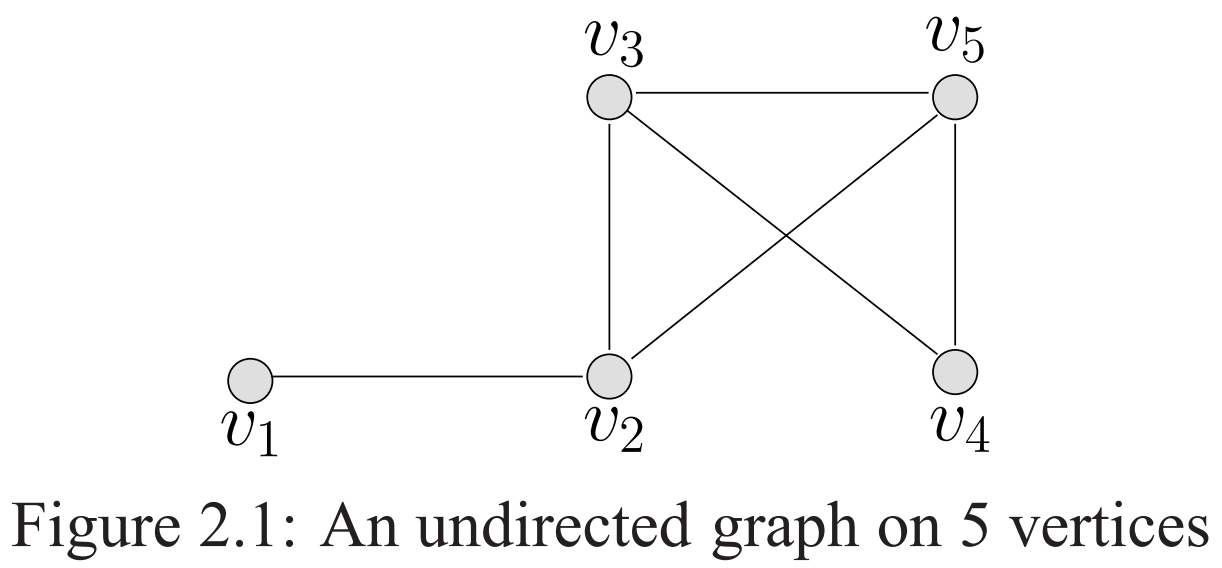
\includegraphics[width=0.8\linewidth]{images/Figure_2_1.png}
    \end{figure}
    \begin{align*}
        V &= \{ v_1, v_2, \dots , v_5 \} \\
        E &= \{ v_1 v_2, v_2 v_3, v_3 v_4, v_3 v_5 , v_2 v_5, v_4 v_5\}
    \end{align*}
    \item The {\color{red}neighborhood} $N(i) \subseteq V$ of the vertex $v_i$ is defined as $N(i) = \{v_j \in V | v_i v_j \in E\}$. $N(i)$ is the set of all vertices that are {\color{red}adjacent} to $v_i$.
    \begin{itemize}
        \item If $v_{\color{red}j} \in N({\color{blue}i})$, then $v_{\color{blue}i} \in N({\color{red}j})$ 
    \end{itemize}
    \item A {\color{blue}path} of length ${\color{red}m}$ in $\mathcal{G}$ is given by a sequence of distinct vertices $v_{i_0}, v_{i_1},\dots , v_{i_{\color{red}m}}$.
\end{itemize}
% \section{Week 3}
\colorbox{black}{\textbf{\color{white}Governing equations}}

\begin{itemize}
    \item Governing equations are mathematical statements of the \textbf{{\color{red}conservation laws of physics}}:
    \begin{itemize}
        \item \textbf{\color{orange}Conservation of Mass} (a.k.a. Continuity Equation)
        \begin{itemize}
            \item Mass is conserved for the fluid
        \end{itemize}
        \item \textbf{\color{orange}Conservation of Momentum} (a.k.a. Newton's 2nd Law / the Navier-Stokes Equation)
        \begin{itemize}
            \item The rate of change of momentum equals the sum of forces acting on the fluid
        \end{itemize}
        \item \textbf{\color{orange}Conservation of Energy} (a.k.a. 1st Law of Thermodynamics)
        \begin{itemize}
            \item The rate of change of energy equals the sum of rate of heat addition to and the rate of work done on the fluid
        \end{itemize}
        \item \textbf{\color{orange}Species Transport Equation} (a.k.a. Principal of Species Conservation)
    \end{itemize}
\end{itemize}

\colorbox{black}{\textbf{\color{white}Auxiliary / Completion Equations}}
\begin{itemize}
    \item Completion equations are relations needed to complete data to solve the \textbf{governing equations}
    \item Examples:
    \begin{itemize}
        \item Equations of State: Gas Law, Density Relations
        \item Constitutive Relations: Viscosity, Turbulence Models
        \item Fluid Property Relations: Conductivity, Specific Heat
        \item Initial / Boundary Conditions
        \item Equations specific to a given problem
    \end{itemize}
\end{itemize}

\colorbox{black}{\textbf{\color{white}Substantial Derivative}}
\begin{itemize}
    \item Substantial Derivative is also called \textbf{\color{orange}total derivative}, \textbf{\color{red}convective derivative}, \textbf{\color{blue}material derivative}, or \textbf{\color{teal}substantive derivative.}
    \begin{itemize}
        \item Substantial derivative $\frac{D\phi}{Dt}$ is the time rate of change following a moving fluid element
        \item Partial derivative $\frac{\partial \phi}{\partial t}$ is the time rate of change  at a fixed location
    \end{itemize}
    \item As a math concept, the substantial derivative is defined as
    \begin{equation*}
        \frac{D(\cdot)}{Dt} = \frac{\partial (\cdot)}{\partial t} + \bm{V}\cdot \frac{\partial (\cdot )}{\partial \bm{x}}
    \end{equation*}
    For example, if temperature $T$ is a function of time and spatial coordinates, then the material derivative of $T(t,x,y,z)$ is,
    \begin{align*}
        \frac{DT}{Dt} &= \frac{\partial T}{\partial t} + \bm{V} \cdot \nabla T \\
        &= \frac{\partial T}{\partial t} + u \frac{\partial T}{\partial x} + v \frac{\partial T}{\partial y} + w \frac{\partial T}{\partial z} \\
        &= \frac{\partial T}{\partial t} + \left(\frac{\partial T}{\partial x}\right)\left(\frac{\partial x}{\partial t}\right) + \left(\frac{\partial T}{\partial y}\right)\left(\frac{\partial y}{\partial t}\right)\\
        &+\left(\frac{\partial T}{\partial z}\right)\left(\frac{\partial z}{\partial t}\right) \\
        &\equiv \left.\left.\frac{d}{dt}\right[T(t,x,y,z)\right]
    \end{align*}
    \item For a general variable property \textbf{per unit mass} denoted as $\phi$, we have the \textbf{\color{orange}conservative form} of general variable property equation:
    \begin{equation*}
        \frac{D\phi }{D t} = \frac{\partial \phi}{\partial t} + u \frac{\partial \phi}{\partial x} + v \frac{\partial \phi}{\partial y} + w \frac{\partial \phi}{\partial z}
    \end{equation*}
    if $\phi$ is in \textbf{per unit volume}, we have the \textbf{\color{orange}non-conservative form}:
    \begin{equation*}
        \rho\frac{D\phi }{D t} = \rho \frac{\partial \phi}{\partial t} + \rho u \frac{\partial \phi}{\partial x} + \rho v \frac{\partial \phi}{\partial y} + \rho w \frac{\partial \phi}{\partial z}
    \end{equation*}
    \item Only the \textbf{\color{orange}non-conservative form} of the general variable property equation is used to derive the momentum theorem.
\end{itemize}

\colorbox{black}{\textbf{\color{white}Continuity Equation / Mass Conservation}}
\begin{itemize}
    \item Developed from the concept: 
    \begin{equation*}
        \frac{\partial m}{\partial t}= \sum_{\text{in}}\dot{m} - \sum_{\text{out}}\dot{m}
    \end{equation*}
    \item \colorbox{orange}{\textbf{\color{white}General Form:}}
    \begin{align*}
        &\frac{\partial \rho}{\partial t} = - \frac{\partial (\rho u)}{\partial x} - \frac{\partial (\rho v)}{\partial v} - \frac{\partial (\rho w)}{\partial z} \\
        \text{or }\; &\frac{\partial \rho}{\partial t} + \frac{\partial (\rho u)}{\partial x} + \frac{\partial (\rho v)}{\partial v} + \frac{\partial (\rho w)}{\partial z} = 0
    \end{align*}
    \item \colorbox{orange}{\textbf{\color{white}Vector Form:}}
    \begin{equation*}
        \frac{\partial \rho}{\partial t} + \nabla \cdot (\rho \bm{V}) = 0
    \end{equation*}
    \item \colorbox{teal}{\textbf{\color{white}Simplifications}}
    \begin{itemize}
        \item When the flow is \textbf{\color{red}steady state}, the partial derivative w.r.t. time is zero, leaving
        \begin{align*}
            {\color{red}\cancelto{0}{\color{black}\frac{\partial \rho}{\partial t}}} + \nabla \cdot (\rho \bm{V}) &= 0
        \end{align*}
        \item For an \textbf{\color{purple}incompressible fluid}, we have $\rho =$ constant. Hence, the derivative w.r.t. time is zero and $\rho$ can be factored out the partial derivatives w.r.t. space, leaving
        \begin{align*}
            \frac{\partial u}{\partial x} + \frac{\partial  v}{\partial y} + \frac{\partial w}{\partial z} &= 0 \\
            \nabla \cdot \bm{V} &= 0
        \end{align*}
    \end{itemize}
    \item \colorbox{teal}{\textbf{\color{white}Separation of Density \& Velocity Vectors}}
    \begin{itemize}
        \item Using the product rule, the general form of continuity equation becomes,
        \begin{align*}
            {\color{blue}\underbrace{\frac{\partial \rho}{\partial t} + \bm{V}\cdot \nabla \rho}_{:=\frac{D\rho}{Dt}}} + \rho (\nabla \cdot \bm{V}) &= 0
        \end{align*}
        \item If the material is incompressible, then $\rho$ cannot change, so $\frac{D\rho}{Dt}$ must be zero. Thus,
        \begin{equation*}
            \rho (\nabla \cdot \bm{V}) = 0
        \end{equation*}
    \end{itemize}
\end{itemize}



\colorbox{black}{\textbf{\color{white}Key Properties of Momentum Equation}}
\begin{itemize}
    \item A moving fluid element experiences three types of force: \textbf{\color{blue}body forces}, \textbf{\color{red}surface forces}, \textbf{external forces}.
    \item \textbf{\color{blue}Body forces} are due to \textbf{\color{teal}external source}, e.g. gravitational forces, magnetic or electrical forces.
    \item \textbf{\color{red}Surface forces} are due to surface stresses acting on the control volume, which include normal stress $\sigma_{xx}$ and tangential stresses $\tau_{yx}$ and $\tau_{zx}$. 
    \begin{itemize}
        \item Normal stresses are caused by pressure p
        \item Tangential stresses are caused by viscosity. For Newtonian fluids, by Newton's Law of Viscosity, the tangential stresses can be related to linear deformation by the \textbf{\color{orange}first dynamic viscosity constant $\mu$}, and to the volumetric deformation using the \textbf{\color{orange}second dynamic viscosity constant $\lambda$}:
        \begin{align*}
            \tau_{xx} &= {\color{red}2 \mu \frac{\partial u}{\partial x} }+ \lambda \left[ \frac{\partial u}{\partial x} + \frac{\partial v}{\partial y} + \frac{\partial w}{\partial z} \right] \\
            \tau_{yy} &= {\color{red}2 \mu \frac{\partial v}{\partial y}} + \lambda \left[ \frac{\partial u}{\partial x} + \frac{\partial v}{\partial y} + \frac{\partial w}{\partial z} \right] \\
            \tau_{zz} &= {\color{red}2 \mu \frac{\partial w}{\partial z} } + \lambda \left[ \frac{\partial u}{\partial x} + \frac{\partial v}{\partial y} + \frac{\partial w}{\partial z} \right] \\
            \tau_{{\color{red}x}{\color{blue}y}} &= \tau_{yx} = \mu \left( \frac{\partial {\color{blue}v}}{\partial {\color{red}x}} + \frac{\partial {\color{red}u}}{\partial {\color{blue}y}} \right) \\
            \tau_{{\color{red}x}{\color{blue}z}} &= \tau_{zx} = \mu \left( \frac{\partial {\color{blue}w}}{\partial {\color{red}x}} + \frac{\partial {\color{red}u}}{\partial {\color{blue}z}} \right) \\
            \tau_{{\color{red}y}{\color{blue}z}} &= \tau_{zy} = \mu \left( \frac{\partial {\color{blue}w}}{\partial {\color{red}y}} + \frac{\partial {\color{red}v}}{\partial {\color{blue}z}} \right)
        \end{align*}
        \item Stokes Hypothesis: $\lambda = -\frac{2}{3} \mu$ (good approximation for gases)
        \item Kinematic viscosity: $\nu = \frac{\mu}{\rho}$
    \end{itemize}
\end{itemize}



\colorbox{black}{\textbf{\color{white}Navier-Stokes Equation / Momentum Equation}}
\begin{itemize}
    \item The following form is for a \textbf{\color{red}Newtonian fluid} reaching \textbf{\color{orange}steady state (constant fluid properties)} in the \textbf{\color{teal}absence of body forces}:
    \begin{align*}
        \underbrace{\frac{D{\color{red}u}}{Dt}}_{\text{accel.}} &= \underbrace{\frac{\partial {\color{red}u}}{\partial t}}_{\text{local accel.}} + \underbrace{u \frac{\partial {\color{red}u}}{\partial x} + v \frac{\partial {\color{red}u}}{\partial y} + w \frac{\partial {\color{red}u}}{\partial z}}_{\text{advection}} \\
        &= - \underbrace{\frac{1}{\rho}\frac{\partial p}{\partial {\color{red}x}}}_{\text{pressure gradient}} + \underbrace{\nu \left[ \frac{\partial^2 {\color{red}u}}{\partial x^2} + \frac{\partial^2 {\color{red}u}}{\partial y^2} + \frac{\partial^2 {\color{red}u}}{\partial z^2} \right]}_{\text{diffusion}} \\
        &= \frac{1}{\rho}\frac{\partial p}{\partial {\color{red}x}} + \nu \nabla^2 {\color{red}u} \\
        \\
        \frac{D{\color{red}v}}{Dt} &= \frac{\partial {\color{red}v}}{\partial t} + u \frac{\partial {\color{red}v}}{\partial x} + v \frac{\partial {\color{red}v}}{\partial y} + w \frac{\partial {\color{red}v}}{\partial z} \\
        &= - \frac{1}{\rho}\frac{\partial p}{\partial {\color{red}y}} + \nu \left[ \frac{\partial^2 {\color{red}v}}{\partial x^2} + \frac{\partial^2 {\color{red}v}}{\partial y^2} + \frac{\partial^2 {\color{red}v}}{\partial z^2} \right]\\
        \\
        \frac{D{\color{red}w}}{Dt} &= \frac{\partial {\color{red}w}}{\partial t} + u \frac{\partial {\color{red}w}}{\partial x} + v \frac{\partial {\color{red}w}}{\partial y} + w \frac{\partial {\color{red}w}}{\partial z} \\
        &= - \frac{1}{\rho}\frac{\partial p}{\partial {\color{red}z}} + \nu \left[ \frac{\partial^2 {\color{red}w}}{\partial x^2} + \frac{\partial^2 {\color{red}w}}{\partial y^2} + \frac{\partial^2 {\color{red}w}}{\partial z^2} \right]
    \end{align*}
    Combining equations in the three directions give the succinct form of:
    \begin{align*}
        \frac{D\bm{V}}{Dt} &= -\frac{1}{\rho} \nabla p + \nu \nabla^2 \bm{V}\\
        \rho \frac{D\bm{V}}{Dt} &= - \nabla p + \mu \nabla^2 \bm{V}
    \end{align*}
    \item For \textbf{\color{orange}steady flow}, the local acceleration terms are zero. The NS equation can be reduced to
    \begin{equation*}
        \rho (\bm{V}\cdot \nabla)\bm{V} = -\nabla p + \mu \nabla^2 \bm{V}
    \end{equation*}
    \item Meaning of each terms:
    \begin{itemize}
        \item \textbf{\color{red}Local acceleration / Local derivative}: 
        \begin{itemize}
            \item $\frac{\partial u}{\partial t}$, $\frac{\partial v}{\partial t}$, $\frac{\partial w}{\partial z}$
            \item time-dependent unsteady term
        \end{itemize}
        \item \textbf{\color{teal}Advection / Convection term}
        \begin{itemize}
            \item e.g. $u \frac{\partial u}{\partial x} + v \frac{\partial u}{\partial y} + w \frac{\partial u}{\partial z}$
            \item Represent inertial force of the fluid flow
            \item $u \frac{\partial u}{\partial x} = $ acceleration due to motion along x-axis
            \item $v \frac{\partial u}{\partial y} = $ acceleration due to motion along y-axis
        \end{itemize}
        \item \textbf{\color{blue}Diffusion term}
        \begin{itemize}
            \item e.g. $\nu \nabla^2 \bm{V}$
            \item Represent diffusion of fluid properties (in this case, the viscous force)
        \end{itemize}
        \item \textbf{\color{olive}Source term}
        \begin{itemize}
            \item Generation and dissipation term for the transport properties
            \item Since we assume that there is not acting body force, the momentum of the fluid is driven by pressure gradient
        \end{itemize}
    \end{itemize}
    \item Number of unknowns:
    \begin{itemize}
        \item There are 4 equations (3 equations from Navier-Stokes for velocity components and 1 from Continuity Equation)
        \item 6 unknowns: 
        \begin{itemize}
            \item Three velocity components: $u$, $v$, $w$;
            \item density: $\rho$;
            \item viscosity: $\nu$;
            \item thermodynamic pressure: $p$
        \end{itemize}
    \end{itemize}
\end{itemize}

\colorbox{black}{\textbf{\color{white}Assumptions Enabled by Incompressible Flow}}
\begin{itemize}
    \item A incompressible flow is defined as the one in which $\nabla \cdot \bm{V} = 0$, which is equivalent to $\frac{D\rho}{Dt} = 0$
    \item \textbf{\color{teal}It is not necessarily true} that $\frac{D\rho}{Dt}=0$ implies both $\frac{\partial \rho}{\partial t}=0$ and $\nabla \rho = 0$ independently. $\frac{D\rho}{Dt}=0$ Only implies that the sum of these two terms are zero. 
    \begin{itemize}
        \item An example: Consider $\rho(x,t)=x-at$ where $a = \frac{\partial x}{\partial t}= u$.
        \begin{align*}
            \frac{D\rho}{Dt} &= \frac{\partial \rho}{\partial t} + \bm{V}\cdot \nabla \rho \\
            &= -a + \begin{bmatrix}
                u \\
                {\color{red}\cancelto{0}{\color{black}v}} \quad \\
                {\color{red}\cancelto{0}{\color{black}w}} \quad
            \end{bmatrix} \cdot \begin{bmatrix}
                \frac{\partial \rho}{\partial x} \\
                \frac{\partial \rho}{\partial y} \\
                \frac{\partial \rho}{\partial z} 
            \end{bmatrix} \\
            &= -a +u \cdot 1 \\
            &= -a + a =0
        \end{align*}
    \end{itemize}
    \item For a \textbf{\color{red}homogeneous} incompressible flow, which means that it has constant density throughout, i.e. $\rho =$ constant, we have $\frac{\partial \rho}{\partial t}=0$ and $\nabla \rho = 0$.
\end{itemize}

% \section{Week 4}
\colorbox{black}{\textbf{\color{white}Conservation of Energy / Energy Equation}}
\begin{itemize}
    \item \textbf{\color{orange}Energy Equation} is the application of the \textbf{\color{teal}First law of thermodynamics} to a moving fluid element (control volume). Because the \textbf{\color{teal}First Law} only applies to \textbf{\color{red}equilibrium states}, we assume the fluid passes through a number of \textbf{\color{red}quasi-equilibrium states}.
    \item The Energy equation can be expressed as:
    \begin{align*}
        \begin{pmatrix}
            \text{Temporal change in}\\
            \text{energy inside CV}
        \end{pmatrix} &= \underbrace{\sum \begin{pmatrix}
            \text{Energy in and out} \\
            \text{due to \textbf{\color{red}fluid flow}}
        \end{pmatrix}}_{:= d\dot{E}} \\
        &- \underbrace{\sum \begin{pmatrix}
            \text{Energy in and out} \\
            \text{due to \textbf{\color{red}heat transfer}}
        \end{pmatrix}}_{:= d\dot{Q}} \\
        &+ \underbrace{\sum \begin{pmatrix}
            \text{Work per time done by} \\
            \text{pressure and stresses on CV}
        \end{pmatrix}}_{:=d\dot{A}} \\
        &+ \underbrace{\sum \begin{pmatrix}
            \text{External energy input} \\
            \text{e.g. radiation, combustion}
        \end{pmatrix}}_{:=\dot{q}_s} \\
        &+ \sum \begin{pmatrix}
            \text{Work per time done} \\
            \text{by body force }\;\bm{f} \\
        \end{pmatrix}
    \end{align*}
    \begin{itemize}
        \item \colorbox{orange}{\textbf{\color{white}Temporal change in energy inside CV}}
        \begin{itemize}
            \item Equals to the sum of rate of change of internal energy and kinetic energy
            \begin{alignat*}{2}
                &\text{IE} = \rho \, e \cdot d\volume \qquad && \left[\frac{\text{kg}}{m^3}\cdot \frac{J}{\text{kg}}\cdot m^3\right]=[J] \\
                &\text{KE} = \frac{1}{2}\rho \bm{V}^2 \cdot d\volume \qquad && \left[\frac{\text{kg}}{m^3}\cdot m^3 \cdot \frac{m^2}{s^2}\right]=[J] \\
                & \text{where }d\volume = dx \, dy \,dz
            \end{alignat*}
            \begin{equation*}
                \begin{pmatrix}
                    \text{Temporal change in}\\
                    \text{energy inside CV}
                \end{pmatrix} = \frac{\partial \left[\rho \cdot \left( e + \frac{\bm{V}^2}{2} \right)\right]}{\partial t} \cdot d\volume
            \end{equation*}
        \end{itemize}
        \item \colorbox{orange}{\textbf{\color{white}Energy in and out due to fluid flow}}
        \begin{align*}
            d\dot{E} &= - \left[\frac{\partial \left[\rho\left(e+\frac{\bm{V}^2}{2}\right)\cdot {\color{red}u}\right]}{\partial {\color{red}x}}\right.\\
            &+\frac{\partial \left[\rho\left(e+\frac{\bm{V}^2}{2}\right)\cdot {\color{red}v}\right]}{\partial {\color{red}y}}\\
            &+ \left.\frac{\partial \left[\rho\left(e+\frac{\bm{V}^2}{2}\right)\cdot {\color{red}w}\right]}{\partial {\color{red}z}}\right]\cdot d\volume
        \end{align*}
        \item \colorbox{orange}{\textbf{\color{white}Energy in and out due to heat transfer}}
        \begin{itemize}
            \item By Fourier's Law of Heat Conduction, the heat fluxes can be related to the local temperature gradient
        \end{itemize}
        \begin{alignat*}{2}
            & \dot{q} := \text{Heat Flux} \qquad &&\left[ \frac{W}{m^2} \right] \\
            & k := \text{Thermal conductivity} \qquad && \left[ \frac{W}{m\cdot K} \right]
        \end{alignat*}
        \begin{equation*}
            d\dot{Q} = \left[\frac{\partial}{\partial x}\left(k \frac{dT}{dx}\right) + \frac{\partial}{\partial y}\left(k \frac{dT}{dy}\right) + \frac{\partial}{\partial z}\left(k \frac{dT}{dz}\right)\right] \cdot d\volume
        \end{equation*}
        \item \colorbox{orange}{\textbf{\color{white}Work per time done by pressure and stresses on CV}} 
        \begin{align*}
            d\dot{A} &= \left[ - \underbrace{\frac{\partial (p {\color{red}u})}{\partial {\color{red}x}}}_{\text{by pressure}}+ \underbrace{\color{orange}\frac{\partial (\sigma_{xx} u)}{\partial x} + \frac{\partial (\tau_{xy} v)}{\partial x} + \frac{\partial (\tau_{xz} w)}{\partial x}}_{\text{by stresses}} \right] d\volume \\
            &+\left[ - \underbrace{\frac{\partial (p {\color{red}v})}{\partial {\color{red}y}}}_{\text{by pressure}}+ \underbrace{\color{orange}\frac{\partial (\sigma_{yy} v)}{\partial y} + \frac{\partial (\tau_{yx} v)}{\partial y} + \frac{\partial (\tau_{yz} w)}{\partial y}}_{\text{by stresses}} \right] d\volume \\
            &+\left[ - \underbrace{\frac{\partial (p {\color{red}w})}{\partial {\color{red}z}}}_{\text{by pressure}}+ \underbrace{\color{orange} \frac{\partial (\sigma_{zz} w)}{\partial z} + \frac{\partial (\tau_{zx} v)}{\partial z} + \frac{\partial (\tau_{zy} w)}{\partial z}}_{\text{by stresses}} \right] d\volume \\
            d\dot{A} &= - \frac{\partial (p u)}{\partial x} - \frac{\partial (p v)}{\partial y} - \frac{\partial (p w)}{\partial z} + {\color{orange}\Phi}
        \end{align*}
        \begin{itemize}
            \item Dissipation function ${\color{orange}\Phi}$ represents the energy due to deformation work done on the fluid.
            \item ${\color{orange}\Phi}$ can also be expressed in terms of velocity components:
            \begin{align*}
                {\color{orange}\Phi} &= 2\mu  \left[ \left( \frac{\partial u}{\partial x} \right)^2 + \left( \frac{\partial v}{\partial y} \right)^2 + \left( \frac{\partial w}{\partial z} \right)^2 \right] \\
                &+ \mu \left( \frac{\partial v}{\partial x} +  \frac{\partial u}{\partial y} \right)^2 + \mu \left( \frac{\partial w}{\partial y} + \frac{\partial v}{\partial z} \right)^2 + \mu \left( \frac{\partial u}{\partial z} +  \frac{\partial w}{\partial x} \right)^2 \\
                &- \frac{2}{3}\mu  \cdot \left( \frac{\partial u}{\partial x} + \frac{\partial v}{\partial y} + \frac{\partial w}{\partial z} \right)^2
            \end{align*}
        \end{itemize}
        \item External energy input: $\rho \cdot \bm{\dot{q}_s}$
        \item Work per time done by body force: $\bm{f} \cdot \bm{V}$
        \begin{itemize}
            \item Gravitational force is usually regarded as a body force and its effects of potential energy changes as a source term
        \end{itemize}
    \end{itemize}
    \item \colorbox{orange}{\textbf{\color{white}Putting it all together ...}}
    \begin{itemize}
        \item Expanded Form of Energy Equation
        \begin{align*}
            & {\color{blue}\rho \left( \frac{\partial e}{\partial t} + u \frac{\partial e}{\partial x} + v \frac{\partial e}{\partial y} + w \frac{\partial e}{\partial z} \right) } = \\ 
            & {\color{red}\left[\frac{\partial}{\partial x}\left(k \frac{dT}{dx}\right) + \frac{\partial}{\partial y}\left(k \frac{dT}{dy}\right)+ \frac{\partial}{\partial z}\left(k \frac{dT}{dz}\right)\right]} \\
            & {\color{orange}- \frac{\partial (p u)}{\partial x} - \frac{\partial (p v)}{\partial y} - \frac{\partial (p w)}{\partial z}} + {\color{orange}\Phi} \\
            &+ \bm{f}\cdot \bm{V} + \rho \cdot \bm{\dot{q}_s}
        \end{align*}
        \item Succinct Form of Energy Equation
        \begin{align*}
            {\color{blue}\rho \frac{ De}{Dt}} = {\color{red}\nabla \cdot (k \nabla T)} - {\color{orange}p (\nabla \cdot \bm{V})} + {\color{orange}\Phi} + \bm{f}\cdot \bm{V} + \rho \cdot \bm{\dot{q}_s}
        \end{align*}
    \end{itemize}
    \item \colorbox{orange}{\textbf{\color{white}Further Simplifications}}
    \begin{itemize}
        \item Unless the engineering problem explicitly states, we assume that $\bm{f}\cdot \bm{V} = 0$ and $\rho \cdot \bm{\dot{q}_s} = 0$.
        \item For incompressible flow, we have ${\color{orange}p(\nabla \cdot \bm{V})}=0$.
        \item For ideal gases, we can relate the internal energy $e$ with enthalpy $h$:
        \begin{align*}
            h &= e + \frac{p}{\rho} = C_p \cdot T \\
            \therefore \; e &= C_p \cdot T - \frac{p}{\rho} \\
            \text{or } \; e &= C_v \cdot T
        \end{align*}
        \begin{itemize}
            \item Energy equation for ideal gases using $C_p$:
            \begin{align*}
                \rho C_p \frac{DT}{Dt} &= \nabla \cdot (k\nabla T) + \frac{Dp}{Dt} + \Phi
            \end{align*}
            \item Energy equation for ideal gases using $C_v$:
            \begin{align*}
                \rho C_v \frac{DT}{Dt} &= \nabla \cdot (k \nabla T) - p (\nabla \cdot \bm{V}) + \Phi
            \end{align*}
        \end{itemize}
    \end{itemize}
    \item For most practical fluid engineering problems, the local time derivative of pressure $\frac{\partial p}{\partial t}$ (in the term $\frac{Dp}{Dt}$ if we use the $C_p$ formulation) and the dissipation function $\Phi$ can be neglected. The Energy Equation is reduced to
    \begin{align*}
        \frac{DT}{Dt} &= \frac{\partial T}{\partial t} + \underbrace{u \frac{\partial T}{\partial x} + v \frac{\partial T}{\partial y} + w \frac{\partial T}{\partial z}}_{\text{advection}} \\
        &= \frac{k}{\rho C_p} \underbrace{\left[ \frac{\partial^2 T}{\partial x^2} + \frac{\partial^2 T}{\partial y^2} + \frac{\partial^2 T}{\partial z^2} \right]}_{\text{diffusion}} \\
        &= \frac{k}{\rho C_p} (\nabla^2 \cdot T)
    \end{align*}
\end{itemize}

\colorbox{black}{\textbf{\color{white}Non-dimensionalization}}

This topic is more question-related. Will be summarized in the last part.
% \section{Week 5}

Content in Week 5 does not weigh as heavy as other contents, so the summary will be short.

\vspace{0.5cm}

\colorbox{black}{\textbf{\color{white}Boundary Conditions (BCs)}}
\begin{itemize}
    \item \textbf{\color{red}Boundary conditions} (a.k.a. the \textbf{\color{red}initial conditions}) are the \textbf{\color{blue}real driver} for CFD solutions because they strongly dictate the particular solutions obtained from the governing equations.
\end{itemize}

\colorbox{black}{\textbf{\color{white}Momentum Boundary Conditions}}
\begin{itemize}
    \item No-slip wall
    \begin{itemize}
        \item A BC on a solid surface for viscous flows which assumes \textbf{\color{teal}zero relative velocity} between the surface and the fluid immediately at the surface
        \item If the surface is stationary,
        \begin{equation*}
            u=v=w=0
        \end{equation*}
    \end{itemize}
    \item Inflow condition
    \begin{itemize}
        \item This BC is needed because solutions of the governing equations require at least one velocity component
        \item E.g. $u=f$ and $v=w=0$ at the inflow boundary ($f$ can be constant or velocity profile)
    \end{itemize}
    \item Outflow condition
    \begin{itemize}
        \item This BC needs to positioned at locations where the flow is \textbf{\color{red}unidirectional} and where \textbf{\color{blue}surface stresses taken known values}.
        \item In a fully-developed flow exiting the channel, there is no change in velocity component in the direction across the boundary
        \item To satisfy stress continuity, the shear forces along the surface are taken to be zero:
        \begin{equation*}
            \frac{\partial u}{\partial n} = \frac{\partial v}{\partial n} = \frac{\partial w}{\partial n} = 0
        \end{equation*}
    \end{itemize}
\end{itemize}


\colorbox{black}{\textbf{\color{white}Validation and Verification}}
\begin{itemize}
    \item  Verification
    \begin{itemize}
        \item Check whether the conceptual model is programmed correctly into a computer model
        \item Are we solving it numerically accurately?
        \item Provide evidence that the equations are solved right:
        \begin{itemize}
            \item Do we have Mesh Sensitivity / Grid Independence/Convergence? Can be examined via key functionals plots (functionals against number of elements) or by grid convergence index (GCI) which quantifies for the grid error
            \item How about grid quality? 
            \item Is the residue target (convergence criterion) sufficient?
            \item Is the spatial and temporal discretization sufficient? Are there enough grid points / enough timesteps?
            \item Is the chosen discretization scheme accurate?
        \end{itemize}
    \end{itemize}
    \item Validation
    \begin{itemize}
        \item Check whether the computer model reflects the actual physical phenomenon.
        \item Provide evidence the right model is solved:
        \begin{itemize}
            \item Are the BCs similar to the actual experimental conditions? Are the boundaries positioned in the right location (e.g. far field boundaries)?
            \item Is the geometry of bluff body correct?
            \item Is the right turbulence model being used?
            \item What is the error between the simulated solutions and the experimental data?
        \end{itemize}
    \end{itemize}
\end{itemize}

\colorbox{black}{\textbf{\color{white}Types of Errors}}
\begin{itemize}
    \item Acknowledged error
    \begin{itemize}
        \item Can be identified with strategic approaches (e.g. approximation, discretization)
    \end{itemize}
    \item Unacknowledged error
    \begin{itemize}
        \item Cannot be identified with strategic approaches (i.e. programming error) 
    \end{itemize}
    \item Truncation error
    \begin{itemize}
        \item When we approximate a PDE by a difference formula, we neglect the Higher Order Term (H.O.T.)
    \end{itemize}
    \item Discretization error
    \begin{itemize}
        \item Difference between exact solution values and those obtained with discretized equations
    \end{itemize}
    \item Round-off error
    \begin{itemize}
        \item Computers use a finite word length of the real numbers, which leads to rounding errors.
    \end{itemize}
\end{itemize}

\colorbox{black}{\textbf{\color{white}Numerical Concepts}}
\begin{itemize}
    \item Consistency
    \begin{itemize}
        \item If the algebraic equations can be shown to be equivalent to the original governing equations as the grid spacing and time steps tends to zero (i.e. $\Delta x \to 0$ and $\Delta t \to 0$), then the numerical model is consistent.
    \end{itemize}
    \item Convergence 
    \begin{itemize}
        \item The property of a numerical method to produce a solution which approaches the exact solution as the grid spacing tends to zero
    \end{itemize}
    \item Stability
    \begin{itemize}
        \item Associated with the damping of errors in the numerical scheme
    \end{itemize}
    \item Conservativeness
    \begin{itemize}
        \item Ensures global conservation of fluid properties through the domain
    \end{itemize}
    \item Boundedness
    \begin{itemize}
        \item Related to stability - ensures the solution is bounded by maximum and minimum values of the flow variables
    \end{itemize}
    \item Transportiveness
    \begin{itemize}
        \item Accounts for directionality of diffusion and convection flows
    \end{itemize}
\end{itemize}


% \section{Week 6}
Break week, no content delivered.
% \section{Week 7}

\colorbox{black}{\textbf{\color{white}Time-Averaging}}

\begin{itemize}
    \item \colorbox{orange}{\textbf{\color{white}Reynolds-Averaging}}
    \begin{itemize}
        \item A general instantaneous flow property $\phi$ is decomposed into a sum of its steady mean motion $\overline{\phi}$ and a fluctuating / eddy motion $\phi '$
        \begin{align*}
            \phi &= \overline{\phi} + \phi ' \\
            \text{where }\; \overline{\phi} &:= \frac{1}{t_0} \int_{0}^{t_0} \phi \, dt \\
            \overline{\phi '} &:= \frac{1}{t_0} \int_{0}^{t_0} \phi ' \, dt \equiv 0 
        \end{align*}
        where $t_0$ is some sufficiently large time interval greater than the time scales of the slowest variations.
        \item \colorbox{teal}{\textbf{\color{white}Useful Formulae}}
        \begin{alignat*}{3}
            & \overline{\overline{\alpha}} = \overline{\alpha}; \quad && \overline{\alpha+\beta}= \overline{\alpha} + \overline{\beta}; \quad && \overline{\overline{\alpha}\beta} = \overline{\alpha}\overline{\beta}; \\
            & \overline{\alpha \beta} = \overline{\alpha}\overline{\beta} + \overline{\alpha ' \beta '}; \quad && \frac{\overline{\partial \alpha}}{\partial s} = \frac{\partial \overline{\alpha}}{\partial s}; \quad && \overline{\int \alpha \, ds} = \int \overline{\alpha} \, ds \\
            & \rho = \overline{\rho}+ \rho ' \quad && u_i = \overline{u}_i + u_i ' \quad && \overline{\bar{\rho} \bar{\alpha} \beta '} = 0
        \end{alignat*}
        \textbf{\color{red}N.B.} fluctuations in dynamic viscosity $\mu$, thermal conductivity $k$, specific heat $C_p$, and mass diffusivity $D$ are neglected in majority of practical applications.
    \end{itemize}
    \item \colorbox{orange}{\textbf{\color{white}Favre-Averaging}}
    \begin{itemize}
        \item Favre-averaging employs a mass-weighted mean property, viz. $\widetilde{\phi}$
        \begin{alignat*}{2}
            &\widetilde{\phi} = \frac{\overline{\rho \phi}}{\overline{\phi}} \qquad && \phi = \widetilde{\phi} + \phi ''\\
            &\overline{\rho \phi} = \overline{\rho}\widetilde{\phi} + \overline{\rho \phi ''} \qquad && \overline{\rho \phi '' } \equiv 0 \\
            &\rho = \overline{\rho} +\rho ' \qquad && \overline{\rho u_i } = \overline{\rho} \widetilde{u_i}
        \end{alignat*}
    \end{itemize}
\end{itemize}

\colorbox{black}{\textbf{\color{white}Boussinesq Approximation}}
\begin{itemize}
    \item It links the Reynolds stresses to the mean rates of deformation \textbf{\color{red}by assuming that the momentum transferred by the turbulent eddies can be modelled by the eddy viscosities.}
    \begin{alignat*}{2}
        &\text{RANS} \quad && - \overline{\rho} \, \overline{u_i ' u_j '} = \mu_T \left(\frac{\partial \overline{u}_i}{\partial x_j} + \frac{\partial \overline{u}_j}{\partial x_i}\right) - \frac{2}{3} \left(\mu_T \frac{\partial \overline{u}_i}{\partial x_j} + \overline{\rho} k\right)\delta_{ij} \\
        &\text{FANS} \quad && - \overline{\rho} \, \overline{u_i '' u_j ''} = \mu_T \left(\frac{\partial \widetilde{u}_i}{\partial x_j} + \frac{\partial \widetilde{u}_j}{\partial x_i}\right) - \frac{2}{3} \left(\mu_T \frac{\partial \widetilde{u}_i}{\partial x_j} + \overline{\rho} k\right)\delta_{ij} 
    \end{alignat*}
    where $\mu_T$ is the eddy viscosity, $k$ is the turbulent kinetic energy, and $\delta_{ij}$ is the Kronecker Delta
    \item \textbf{\color{orange}Intuitive Interpretation:} If an eddy is more resistant to the departing momentum, then it means that the eddy can take up more viscous force.
    \item The purpose of Boussinesq approximation is to express the resolvable Reynolds stress tensor into a function of the mean flow (which consists of known terms).
\end{itemize}
% \section{Week 8}

\colorbox{black}{\textbf{\color{white}Turbulence Models}}

\begin{itemize}
    \item Standard $k-\varepsilon$, RNG $k-\varepsilon$, Realizable $k-\varepsilon$, Standard $k-\omega$, Transition SST, and Reynold Stress model are RANS-based Model.
    \item Detached Eddy Simulation and Large Eddy Simulation are not RANS based Model.
    \item The most accurate RANS turbulence model in terms of drag coefficient w.r.t. air flowing over a cylinder body is \textbf{\color{orange}Transition SST Model}, which is better in the following aspects:
    \begin{itemize}
        \item convergence and stability
        \item performs better for high speed flows
        \item combines the fine features of both $k-\varepsilon$ and $k-\omega$ models (at free-stream and near wall regions respectively)
        \item Transition SST requires fine mesh near the wall region
    \end{itemize}
\end{itemize}

\colorbox{black}{\textbf{\color{white}Pros \& Cons}}

\begin{itemize}
    \item \colorbox{orange}{\textbf{\color{white}Standard $k-\varepsilon$}}
    \begin{itemize}
        \item {\color{red}Robust, efficient, easy to apply}
        \item {\color{red}Solves better at the free steam}
        \item {\color{blue}Performs poorly for complex flows involving severe pressure gradient, separation, or strong streamline curative}
        \item {\color{blue}Over-predicts the TKE energy at the wall region}
    \end{itemize}
    \item \colorbox{orange}{\textbf{\color{white}RNG $k-\varepsilon$}}
    \begin{itemize}
        \item {\color{red}Enhanced version of standard $k-\varepsilon$ model with additional term in $\epsilon$ equation}, which accounts for interaction between turbulence and mean shear.
        \item {\color{red}Suitable for complex shear flows involving:}
        \begin{itemize}
            \item Strong streamline curvature and rapid strain;
            \item moderate swirl and vortices;
            \item Separated flows;
            \item Wall heat and mass transfer;
        \end{itemize}
        \item {\color{blue}Inappropriate for prediction of round jet flows}
    \end{itemize}
    \item \colorbox{orange}{\textbf{\color{white}Realizable $k-\varepsilon$}}
    \begin{itemize}
        \item {\color{red}Offer same benefits as RNG $k-\varepsilon$}
        \item {\color{red}Better convergence as compared to RNG $k-\varepsilon$}
        \item {\color{red}Includes eddy-viscosity concept}
        \item {\color{red}Suitable for flows involving:}
        \begin{itemize}
            \item Planar and round jets;
            \item \textbf{Rotation and recirculation}
        \end{itemize}
    \end{itemize}
    \item \colorbox{orange}{\textbf{\color{white}Standard $k-\varepsilon$}}
    \begin{itemize}
        \item {\color{red}Superior performance for wall-bounded boundary layer (e.g. flow in pipe)}
        \item {\color{blue}This model under-predicts the TKE energy at the free stream}
    \end{itemize}
    \item \colorbox{orange}{\textbf{\color{white}SST $k-\omega$}}
    \begin{itemize}
        \item {\color{red}Combines the benefits of $k-\varepsilon$ and $k-\omega$ models}
        \item {\color{red}Has a better transition between the free stream and near wall regions}
        \item {\color{blue}Requires mesh resolution / refinement near the wall}
    \end{itemize}
    \item \colorbox{orange}{\textbf{\color{white}Reynolds Stress}}
    \begin{itemize}
        \item {\color{red}Physically the most reliable RANS model}
        \item {\color{red}Suitable for:}
        \begin{itemize}
            \item complex 3D flows with strong streamline curvature;
            \item Strong swirl/rotation
        \end{itemize}
        \item {\color{blue}More CPU time and memory requirement}
    \end{itemize}
\end{itemize}


% \section{Week 9}
\colorbox{black}{\textbf{\color{white}Finite Difference Approximation (FDA)}}

\begin{itemize}
    \item \textbf{\color{red}Taylor series expansion} are used to approximate the partial derivatives. 
    \item Truncation errors exist due to higher order terms are ignored. \textbf{\color{orange}Truncation errors are negligible if the system is stable}.
\end{itemize}

\colorbox{black}{\textbf{\color{white}Finite Difference Methods (FDM)}}
\begin{itemize}
    \item FDMs discretize the domain into a grid. 
    \item Variables are evaluated at the grid points.
    \item FDM is commonly applied to \textbf{\color{red}structured mesh} as it requires a mesh having a high degree of regularity
    \item Pros: FDM allows the use of higher-order differencing approximations which provide a higher degree of accuracy in the solution
    \item \colorbox{teal}{\textbf{\color{white}Approximations of 1st order derivative}}
    \begin{itemize}
        \item \textbf{\color{red}Central Difference}
        \begin{alignat*}{2}
            &\text{Space:} \qquad && \frac{\partial \phi}{\partial x} = \frac{\phi_{i+1,j}-\phi_{i-1,j}}{2\Delta x} + O(\Delta x^2) \\
            &\text{Time:}\qquad && \text{N/A}
        \end{alignat*}
        \item \textbf{\color{red}Forward Difference}
        \begin{alignat*}{2}
            &\text{Space:}\qquad &&\frac{\partial \phi}{\partial x} = \frac{\phi_{i+1,j}-\phi_{i,j}}{\Delta x} + O(\Delta x)\\
            &\text{Time:}\qquad && \frac{\partial \phi }{\partial t} = \frac{\phi_{i,j}^{n+1}-\phi_{i,j}^{n}}{\Delta t} + O(\Delta t)
        \end{alignat*}
        \item \textbf{\color{red}Backward Difference}
        \begin{alignat*}{2}
            &\text{Space:} \qquad && \frac{\partial \phi}{\partial x} = \frac{\phi_{i,j}-\phi_{i-1,j}}{\Delta x} + O(\Delta x) \\
            &\text{Time:} \qquad && \frac{\partial \phi}{\partial t} = \frac{\phi_{i,j}^{n}-\phi_{i,j}^{n-1}}{\Delta t} + O(\Delta t)
        \end{alignat*}
    \end{itemize}
    \item \colorbox{teal}{\textbf{\color{white}Approximation of 2nd order derivative}}
    \begin{itemize}
        \item \textbf{\color{red}Central Difference}
        \begin{alignat*}{2}
            &\text{Space:} \qquad && \frac{\partial^2 \phi}{\partial x^2} = \frac{\phi_{i+1,j}-2\phi_{i,j}+\phi_{i-1,j}}{\Delta x^2} + O(\Delta x^2)
        \end{alignat*}
    \end{itemize}
\end{itemize}

\colorbox{black}{\textbf{\color{white}Finite Volume Methods (FVM)}}

\begin{itemize}
    \item FVMs discretize the domain into a number of contiguous control volumes.
    \item Variables are evaluated at the centroids of CV, and interpolation (a.k.a discretization schemes) is used to obtain variables values at the control volume face. 
    \item FVM can be applied to both \textbf{\color{red}structured} and \textbf{\color{red}unstructured} mesh.
    \item Cons: higher-order ($>$2nd order) differencing approximations are more difficult to obtain.
    \item \colorbox{orange}{\textbf{\color{white}Approximation Schemes of Surface Variables}}
    \begin{figure}[H]
        \centering
        \includegraphics[width=1.0\linewidth]{images/summary_discretization_scheme.png}
    \end{figure}
    \begin{itemize}
        \item \textbf{\color{red}Central Difference}
        \begin{align*}
            \phi_e &= \frac{1}{2} (\phi_P + \phi_E) \\
            \text{where }\; \phi_e &= \text{value at face}\\
            \phi_P &= \text{value at owner cell} \\
            \phi_E &= \text{value at neighbor cell}
        \end{align*} 
        Alternatively, using subscript notations,
        \begin{align*}
            \phi_f &= \frac{1}{2} (\phi_i + \phi_{i+1}) \\
            \text{where }\; \phi_f &= \text{value at face}\\
            \phi_i &= \text{value at owner cell} \\
            \phi_{i+1} &= \text{value at neighbor cell}
        \end{align*} 
        \begin{itemize}
            \item Pros: 2nd order accuracy
            \item Cons: can become unstable; may give large undershoots or overshoots
        \end{itemize}
        \item \textbf{\color{red}Upwind Difference (1st order)}
        \begin{alignat*}{2}
            & \phi_f = \phi_{i} \qquad && F_e > 0 \; \text{(backward)} \\
            & \phi_f = \phi_{i+1} \qquad && F_e < 0 \; \text{(forward)}
        \end{alignat*}
        An example approximating the term $u \frac{\partial T}{\partial x}$:
        \begin{alignat*}{2}
            & \frac{\partial T}{\partial x} = \frac{T_{i}^{n}-T_{i-1}^{n}}{\Delta x} \qquad && \text{if }\; u > 0 \\
            & \frac{\partial T}{\partial x} = \frac{T_{i+1}^{n}-T_{i}^{n}}{\Delta x} \qquad && \text{if }\; u < 0 
        \end{alignat*}
    \end{itemize}
\end{itemize}
% \section{Week 10}

\colorbox{black}{\textbf{\color{white}Von Neumann Stability Analysis}}

\begin{itemize}
    \item \textbf{\color{teal}DuFort-Frankel method (explicit)}, any \textbf{\color{blue}fully implicit ($\theta = 1$) scheme}, and \textbf{\color{orange}semi-implicit Crank-Nicolson ($\theta = 0.5$) scheme} are \textbf{\color{red}unconditionally stable} 
\end{itemize}

difference between consistency, convergence, and stability

For pure convection case, if use FTCS as FDA, the solution is unconditional unstable


\printbibliography


\end{document}